% soctepmlate
% Author: Vojtěch Boček
% Edit by: Jaroslav Páral
% Version: 2018-02-12
% Source code: https://github.com/RoboticsBrno/soctemplate/
% Base on: http://www.jcmm.cz/cz/sablona-soc.html
% License: CC BY 4.0

\documentclass{template/socthesis}

\usepackage{subcaption}
\usepackage{amsmath}
\usepackage{enumitem}

\addbibresource{text.bib}

\titlecz{Modulární stavba soutěžních robotů}
\titleen{Modular construction of competitive robots}
\author{Tomáš Rohlínek}
\field{18} % Obory SOČ: 1 - 18 (http://www.soc.cz/obory-soc/)
\school{Střední průmyslová škola a Vyšší odborná škola Brno, Sokolská, příspěvková organizace}
\mentor{Mgr. Miroslav Burda}
\mentorstatement{Mgr. Miroslava Burdy}

% Změňte, pokud se liší
%\region{Jihomoravský}
\placefooter{Brno 2020}

\begin{document}
	\maketitle
	
	\makecopyrightstatement{V~Drásově}
	
	\makethanks{Děkuji svému vedoucímu Mgr. Miroslavu Burdovi za pomoc, podnětné připomínky a hlavně nekonečnou trpělivost.}
	
	\pagestyle{empty}
	
	\section*{Anotace}
	Cílem této práce je vytvořit sadu univerzálních senzorů pro soutěžní roboty tak, aby jejich instalace, využívání a případná tvorba modulů nových byla co uživatelsky nejpřívětivější.
	
	\subsection*{Klíčová slova}
	robotika; senzory; komunikace; modulární konstrukce
	
	\vspace{20mm}
	
	\section*{Annotation}
	The goal of this work is to create a pack of sensors for competetive robots, while their installation, usage and creation, is as user friendly, as possible. 
	
	\subsection*{Keywords}
	robotics; sensors; communication; modular construction
	
	\newpage
	\pagestyle{plain}
	
	\tableofcontents % vysází obsah
	
	%%% Začátek práce
	\setcounter{figure}{0}
	\setcounter{table}{0}
	\newpage
	
	%%% Úvod
	\chapter*{Úvod}
\addcontentsline{toc}{chapter}{Úvod} % přidá položku úvod do obsahu
%odsazení od vrchu moc velké
V~poslední době se robotické soutěže těší stále většímu zájmu jak veřejnosti, tak konstruktérů.
Mezi v~česku známé robotické soutěže patří například Pražský robotický den\cite{Prague-robotic-day} a Robotiáda\cite{Robotiada}.
Senzory dosahují různé kvality a používají různé komunikační protokoly a sběrnice, což může být problémem pro začínající konstruktéry, kteří se díky nejednotné nabídce musí starat o~věci jako duplicitní adresy na sběrnici, kolize dvou knihoven řídících jednu sběrnici a hardwarové problémy dané sběrnice.

Cílem této práce je těmto začínajícím konstruktérům poskytnou nástroj, který většinu problémů se senzorikou vyřeší za ně, pro pokročilejší konstruktéry pak nabízí úsporu času.
Tito konstruktéři nemusí již senzory, které se neustále opakují, stavět, zapojovat a programovat vždy znovu, ale dostanou do rukou téměř plug-n-play řešení.


\newpage
	
	%%% Jak psát
	\chapter{Běžně používané sběrnice}
Sběrnice dávají jednotlivým modulům možnost vzájemné komunikace.
Často dochází k~záměně pojmu sběrnice a protokol, což je pochopitelné, neboť se mohu v~různých mírách překrývat.
Sběrnicí většinou rozumíme hardwarovou složku komunikace, ta definuje například počet vodičů, napěťové úrovně na těchto vodičích, atd.
Protokolem pak rozumíme formát dat posílaných po sběrnicích.
V~oboru amatérské stavby robotů se v~praxi používá několik sběrnic a protokolů pro získávání dat:
\begin{itemize}
	\item I$^{2}$C
	\item UART
	      \begin{itemize}
		      \item RS-232
		      \item RS-485
	      \end{itemize}
	\item SPI
	\item 1-Wire
	\item Nesběrnicová komunikace
\end{itemize}

\section{I$^{2}$C}
Snad nejpoužívanější sběrnice a protokol zároveň je I$^{2}$C \cite{nxp:UM10204},
také známá jako Inter-Intergrated Circuit\footnote{ Protože je značka I$^{2}$C chráněna, použili ostatní výrobci název TWI, jedná se o~prakticky stejnou sběrnici, pouze pod jiným názvem.}.
Tato sběrnice byla vyvinuta firmou Philips primárně pro připojení periferií, které nevyžadovaly vysoké komunikační rychlosti.
Sběrnice podporuje jak multi-master, tak multi-slave.
Běžná rychlost je 100~kbit/s, ve Fast modu je 400~kbit/s. Novější revize pak umožňují až 5 Mbit/s, s~touto verzí však nemusí být kompatibilní starší zařízení.
I$^{2}$C používá 7-bitovou adresu, což teoreticky znamená, že je na každé sběrnici možno provozovat až 127 zařízení, prakticky je toto číslo značně nižší.
I$^{2}$C využívá TTL.
Maximální délka sběrnice je 1 metr na 100~kBd, sběrnice však nebyla designovaná na provoz po kabelu, jak je zvyklá ji používat většina amatérských nadšenců.

\begin{table}[h]
	
	\centering
	\begin{tabular}{|l|l|l|l|l|} \hline
		Maximální počet zařízení      & 127              \\ \hline
		Maximální délka               & 1~metr           \\ \hline
		Běžná rychlost                & 100~kbit/s        \\ \hline
		Maximální teoretická rychlost & 5~Mbit/s          \\ \hline
		Minimální počet vodičů        & 3~(SDA, SCL, GND) \\ \hline
	\end{tabular}
	\caption{Shrnutí hlavních parametrů I$^{2}$C}
\end{table}



\section{UART}
Další hojně používanou sběrnicí je UART, mezi amatérskou komunitou známá též jako sériová linka.
UART ve skutečnosti není sběrnice jako taková, jedná se spíše o~něco mezi sběrnicí a protokolem.
UART definuje pouze posílaná data (0 a 1), nikoli však způsob jejich posílání či napěťové úrovně sběrnice.
O~to se starají právě jednotlivé implementace\footnote{I přesto se dá UART používat sám o~sobě na TTL (Transistor-Transistor-Logic), v~tom případě je definice napěťových úrovní ponechána jednotlivým zařízením, což může způsobit vzájemnou nekompatibilitu.}.
Nejběžněji používané implementace UARTu jsou:
\subsection{RS-232} % (fold)
RS-232 \cite{RS-232} je implementace UART.
Používá napěťové úrovně +5~V~až +15~V~pro logickou 1 a --5~V~až --15~V   pro~logickou 0, toto platí pro vysílací část.
Přijímací část přidává dvouvoltovou hysterezi kvůli rušení, což znamená +3~V~až +15~V~pro logickou 1 a --3~V~až --15~V~pro logickou 0.
RS-232 potřebuje společnou GND.
\begin{table}[h]
	
	\centering
	\begin{tabular}{|l|l|l|l|l|} \hline
		Maximální počet zařízení      & 2              \\ \hline
		Běžná rychlost                & 115200~baud/9600~baud        \\ \hline
		Maximální teoretická rychlost & 10~Mbit/s       \\ \hline
		Minimální počet vodičů        & 3~(Tx, Rx, GND) \\ \hline
	\end{tabular}
	\caption{Shrnutí hlavních parametrů RS-232}
\end{table}
% subsection RS-232 (end)
\subsection{RS-485}\label{RS-485} % (fold)
RS-485 \cite{RS-485} je další implementace UARTu.
Nepoužívá ale napěťové úrovně oproti společné GND, nýbrž využívá rozdílu napětí na linkách A~a B, ten musí být alespoň 200~mV.
To způsobuje několik věcí:
\begin{itemize}
	\item Pokud vedou obě linky podél sebe, nejlépe jsou-li kroucené, je prakticky nemožné komunikaci zarušit, což je v~prostředí motorů na robotu značná výhoda\footnote{Zároveň to výrazně zvyšuje maximální možnou délku linky, při nižších rychlostech až na 1200~m. Doporučení: rychlost [baud] * vzdálenost [m] $<$ +/- 10$^{8}$.}.  
	\item Není potřeba společná GND.
	\item Pro plný duplexní mód (jedna linka na vysílání a jedna na přijímání) je potřeba dvojnásobný počet vodičů, tedy 4.
\end{itemize}
V~závislosti na použitém převodníku z~UART na RS-485 může být počet zařízení na sběrnici 32 nebo až 128.
\begin{table}[h]
	
	\centering
	\begin{tabular}{|l|l|l|l|l|} \hline
		Maximální počet zařízení      & 32/128              \\ \hline
		Běžná rychlost                & 115200~baud/9600~baud        \\ \hline
		Minimální počet vodičů        & 2 (A, B) \\ \hline
		Maximální vzdálenost		  & 1200~m \\ \hline
	\end{tabular}
	\caption{Shrnutí hlavních parametrů RS-485}
\end{table}
% subsection RS-485 (end)

\section{SPI}
SPI \cite{nxp:AN2847}, neboli Serial Peripherial Interface, je dvoukanálová synchronní multi-slave\footnote{Na sběrnici je naráz připojen pouze jeden master (řídící jednotka) a typem sběrnice omezené množství slave (řízených) zařízení.} sběrnice.
Pro komunikaci využívá 4 vodiče:
\begin{itemize}
		\item MOSI (Master Output Slave Input) -- výstup z~master a vstup do slave
		\item MISO (Master Input Slave Output) -- výstup ze slave a vstup do master
		\item SCK -- hodinový signál
		\item SS (Slave Select) -- tímto pinem nastavujeme, který slave je momentálně aktivní
\end{itemize}
Na straně masteru může pak díky tomu být počet použitých pinů větší (3~+~počet slave zařízení).

Další možná konfigurace je tzv. Daisy-chain, kdy je  MOSI masteru připojeno na MOSI prvního slave zařízení a MISO prvního slave zařízení je připojeno na MOSI dalšího slave zařízení, až MISO posledního slave zařízení je připojeno na MISO masteru.
Tato konfigurace poskytuje snížení počtu vodičů, zároveň ale snižuje i komunikační rychlost, protože informace od prvního slave zařízení musí obejít celý kruh, než se dostanou zpět k~master zařízení.

Nespornou výhodou SPI je její rychlost.
Maximální rychlost není definovaná, aplikace běžně jdou až přes 10~Mb/s.
Nevýhodou může být velký počet vodičů, př použití standartního zapojení.


\section{1-Wire}
1-Wire \cite{one-wire} je sběrnice (a protokol zároveň), která, jak již její název napovídá, potřebuje pouze jeden vodič.
K~tomu potřebuje ještě společnou GND, ale i tak to jsou pouze 2~vodiče, které obsáhnou napájení i komunikaci\footnote{Sběrnici je možno provozovat i na třílinkovém módu.}.
Této typologie se využívá třeba u~kontaktních přístupových čipů.
Sběrnice je také poměrně známá pro svůj CRC součet, který umožňuje kontrolu odeslaných dat.
1-Wire je kompatibilní s~TTL.
Každé zařízení na sběrnici má unikátní neměnnou adresu.


\section{Nesběrnicová komunikace}
Některé senzory nepotřebují posílat velké množství dat, a proto může být lepší nepoužít sběrnici. 
Příkladem takového senzoru může být třeba obyčejné tlačítko.
Některé senzory zmíněné v~další kapitole také používájí tento způsob předávání dat.
Hlavní problém tohoto řešení je především náročnost na čas procesoru a počet vodičů.


	
	%%% Několik formálních pravidel
	\chapter{Běžně používané senzory na soutežních robotech}

Každý robot potřebuje mít způsob interakce s~okolím.
Tuto interakci zajišťují právě senzory.
Naprostá většina amatérských týmů nemá prostor ani pros\-třed\-ky vytvářet vlastní senzory.
Používání průmyslových senzorů je znemožňováno několika faktory.
Zřejmě nejzásadnějším je cena, dále pak jejich velikost a hmotnost způsobená jejich robustností a kvalitou provedení.
Týmy jsou tedy nuceny používat hotové senzorové moduly, o~nichž často nevědí, jaké komponenty obsahují a jak fungují.
Senzory se dají rozdělit do několika kategorií:
\begin{itemize}
    \item Senzory vzdálenosti
        \begin{itemize}
            \item Ultrazvukové senzory
            \item IR senzory
            \item Lidar/Radar/Sonar
        \end{itemize}
    \item Senzory barvy
        \begin{itemize}
            \item Black-white senzory
            \item RGB senzory
            \item Kamery
        \end{itemize}
    \item Senzory pohybu
        \begin{itemize}
            \item Akcelerometry
            \item Gyroskopy
            \item Enkodéry
            \item Kompasy
        \end{itemize}
    \item Komplexní polohové senzory
\end{itemize}

\section{Senzory vzdálenosti}

Senzory pro zjišťování vzdálenosti dodávájí robotovi poměrně primitivním způsobem schopnost přibližně určit svou polohu na základě vzdáleností od okolních objektů.
Podmínky pro jejich použití jsou však často velmi specifické a nedají se proto samy o~sobě použít pro přesnější lokalizaci.

\subsection{Ultrazvukové senzory}

Asi nejpoužívanějšími senzory vzdálenosti jsou senzory ultrazvukové.
Ty fungují na principu vyslání ultrazvuového pulzu a čekání na jeho návrat.

Nejběžněji používaný z~nich je HC-SR04~\cite{hc-sr04}. 
Ten obsahuje ultrazvukový přijímač a vysílač, spolu s~dodatečnou elektronikou.
Má čtyři vývody: 
\begin{table}[h]
	
	\centering
	\begin{tabular}{|l|l|l|l|l|} \hline
		GND & společná zem/-   \\ \hline
		VCC/5~V~& napájení 5~V/+  \\ \hline
		Echo & Návrat měřené vzdálenosti   \\ \hline
		Trig & Spouštění meření \\ \hline
    \end{tabular}
    \caption{Vývody HC-SR04}
\end{table}

Měření započne posláním logické 1 na pin Trig po dobu alespoň 10~$\mathrm{\mu}$s.
Poté, co Trig opět přepneme na logickou 0, vyšle senzor 8 40-ti kHz pulzů, zárověň nastaví na pinu Echo logickou 1.
Po přijetí odraženého ultrazvukového signálu je na pinu Echo opět nastavena logická 0.
Mikrokontroleru poté pouze zbýva měřit, jak dlouho byla na pinu Echo logická 1, tento čas pak dosadí do rovnice:
% \begin{center}
%     % \begin{equation}
%     %     $\mathrm{vzdálenost=(naměřený čas*rychlost zvuku)}/2$
%     %     \label{eq: Vzdálenost při měření ultrazvukovým senzorem}
%     % \end{equation}
    
    
% \end{center} 
Senzor je schopen měřit vzdálenosti od 2~cm do 4~m, dělá to při 15$^{\circ}$ úhlu.
Senzor má nevalnou přesnost (+/-~2~cm).
Největší úskalí při používaní tohoto senzoru nastává, pokud je na hřišti více robotů, nebo nesynchronizovaných senzorů, kdy se senzory mohou navzájem rušit.
Další problém může vyvstat při používaní pouze jednoho mikroprocesoru a několika ultrazvukových senzorů, kdy čas potřebný na změření všech senzorů přesáhne únosnou mez, čímž se zásadně prodlouží reakční čas robota.
Tento problém se řeší použitím sekundárního procesoru pro obsloužení měření.


\subsection{IR senzory}
Infračervené senzory fungují vesměs na stejném principu jako ty ultrazvukové, pouze ultrazvukové pulzy jsou nahrazeny infračerveným paprskem.
To s~sebou nese oproti ultrazvuku své výhody i nevýhody.
Hlavní výhodou oproti ultrazvuku je menší pravděpodobnost zarušení ambientním signálem, pokud senzor používá modulovaný signál pro měření. 
Nevýhodou je, že stejně jako ultrazvukové senzory mohou být i infračervené senzory přehlceny, v~tomto případě ale spíše silným ambientním zdrojem, například sluncem, než ostat\-ní\-mi senzory.

Nejpoužívanější IR senzor vzdálenosti je FC-51 \cite{fc-51}, který má oproti HC-SR04 výrazně větší měřící úhlel 35$^{\circ}$ a výrazně menší rozsah měřitelných vzdáleností, konkrétně 2~cm až 30~cm.
Na rozdíl od HC-SR04, který měří plynule na celém rozsahu, měří FC-51 pouze přiblížení pod nastavenou mez, podle toho vrací na výstupu 0 a 1.
Hranice přiblížení je nastavitelná pomocí potenciometru nacházejícím se přímo na senzoru.


\subsection{Lidar/Radar/Sonar}
Tato zařízení obsahují běžné senzory vzdálenosti a pouze přidají možnost pohybu těchto senzorů. 
Místo jednosměrného měření pak vytvaří v~podstatě mapu prostoru.
Lidar používá k~měření laserový, většinou IR, paprsek.
Radar používá rádiové vlny, které mohou částečně pronikat materiály, což umožňuje \uv{vidět} skrz zdi.
Sonar používá k~měření zvukové vlny, což je s~výhodou využíváno hlavně pod vodou, kde se tyto vlny velmi dobře šíří.
Bohužel zatím neexistuje spolehlivá a levná iterace těchto senzorů, která by se dala použít na soutěžních robotech.

\section{Senzory barvy}
Senzory barvy jsou použitelné pouze v~některých soutěžních disciplínách.
Dávají našemu robotovi možnost zjišťovat barvu herních objektů a podložky, což může pomoci jak s~orientací, tak s~plněním herních úkolů.

\subsection{Black-white senzory}
Tyto senzory využívají světelný zdroj, zpravidla IR nebo bílý, v~kombinaci s~plynulým světelným senzorem citlivým na vlnovou délku světla zdroje.
Každá látka v~závislosti na své barvě pohlcuje a odráží světlo jinak, nám poté zbývá pouze změřit, kolik světla se odrazilo.
Senzory tedy defakto neměří, jestli je povrch černý nebo bílý, ale spíše jestli je světlý či tmavý.
Existuje obrovské množství iterací tohoto senzoru -- některé plynulé, jiné digitální s~nastavitelnou hranicí překlopení.
B-W senzory se nejčastěji používají v~soutěžích jako line follower\footnote{Soutěž, ve které se robot pokouší co nejrychleji projet dráhu vyznačenou nejčastěji černou čárou na podložce. V~poslední době se do cesty přidávají také překážky, kterým se robot musí vyhnout.}, kde není potřeba kompletní RGB detekce.

\subsection{RGB senzory}
RGB senzory kombinují více B-W senzorů do jednoho celku.
Existují dvě možnosti, jak toho dosáhnout. 

První možnost používá jeden bílý zdroj světla a více senzorů citlivých na specifické vlnové délky, zpravidla 3 senzory pro RGB, občas se také přidává IR a UV.
Všechny senzory přitom mohou měřit naráz.

Druhá možnost používá jeden senzor se širokým spektrem a více zdrojů světla s~různými barvami vyzařovaného světla, opět se nejčastěji používá RGB a případně se k~tomu přidává UV a IR.
Tato možnost má o~něco pomalejší měření oproti první metodě, neboť zdroje světla se musí ve svícení střídat.

\subsection{Kamery}
Zvláštní případem barevných senzorů jsou kamery.
Ty však vyžadují v~závislosti na způsobu použití poměrně velký výpočetní výkon.
To řeší použití samostatného procesoru pro zpracování obrazu, jako to dělá třeba populární Pixy\cite{pixy}\footnote{Nebo můžeme použít aplikaci ve smartphonu, ty pro podobné aplikace mají výpočetního výkonu dostatek. Některé novější by mohly dokonce spustit nějaké Deep learning algoritmy pro zpracování obrazu.}.

Kamery poskytují výhodu hlavně co se zorného pole a vzdálenosti od povrchu týká, nemusí totiž být na rozdíl od dvou předchozích připevněny do několika milimetrů od měřeného povrchu.

\section{Pohybové senzory} 
Senzory pohybu poskytují robotu schopnost určit, jak se v~prostoru pohybuje, některé přímo a některé nepřímo.
Všechny však vyžadují nějaký způsob přepočtu.
Tyto senzory neposkytují vždy přesné údaje, což není způsobeno přímo senzory, ale spíše typem a nedokonalostmi pohybu, který mají měřit.
Polohové senzory, vyjma enkodérů, se zpravidla nepoužívají samostatně, ale v~celcích.
Například běžně používaný senzor mpu-6050 \cite{mpu6050} spojuje dohromady akcelerometr a gyroskop, zárověň má možnost připojit přímo na sebe kompas, což umožňuje vytvořit 9-osý systém.


\subsection{Akcelerometry}
Akcelerometry měří lineární zrychlení.
Ve větším provedení se jedná o~závaží na pružině, která je na druhé straně uchycená k~pouzdru. 
Lineární zrychlení zjístíme změřením a přepočtem změny délky pružiny, neboli o~kolik se pružina zmáčkla/roztáhla, aby uvedla závaží do stejné rychlosti jako má pouzdro.
V~menším provedení se využívá piezoelektrického jevu pro měření.
Senzor může měnit hodnoty v~závislosti na teplotě, to je potřeba buď kompenzovat ve výpočtu, nebo zanedbat -- v~případě nepotřeby superpřesných údajů \cite{accel}.

\subsection{Gyroskopy}
Gyroskopy měří úhlovou rychlost, případně úhel náklonu.
Ve velkém provedení se jedná o~setrvačník připevněný k~pouzdru způsobem, který umožňuje rotaci v~měřených osách.
Rotující setrvačník si zachová nezávisle na pohybu pouzdra svůj počáteční náklon.
Díky tomu máme referenční objekt, od kterého můžeme měřit náklon.
V~menším provedení se používá několik principů, jeden z~nich je Disk Resonator Gyroscope, který využívá pro měření Coriolisovy síly.
Pro měření všech 3 os je potřeba více gyroskopů
\cite{gyro}
\cite{gyro-2}.

\subsection{Enkodéry}
Enkodéry slouží k~převádění mechanického pohybu kol na elektronický signál.
Enkodéry se dají rozdělit na ty, co se používají přímo na pohonu a na vlečné enkodéry.

Enkodéry umístěny na pohonu zabírají méně místa než ty vlečné. 
Na druhou stranu, pokud proklouzne kolo, či část převodu, nemají to tyto senzory jak zjistit.

Vlečné enkodéry mohou mít problém se změnou směru pohybu.
Nejsou však ovlivněny možným proklouznutím hnacího kola, to proto, že měří pohyb relativně k~podložce, na rozdíl od těch umístěných na pohonu, které měří pohyb relativně k~robotovi.


\subsection{Kompasy}
Stejně jako běžné kompasy se elektronické kompasy používají k~zjištění natočení robota v~magnetickém poli Země.

\section{Komplexní polohové senzory}
Když potřebujeme přesné měření polohy, nestačí nám samostatné senzory, musíme vytvořit větší komplexní celek.
Příklad takového systému je Global Positioning System, nebo jeho alternativy jako GLONASS a Galileo.
Tento systém využívá sadu satelitů, které neustále vysílají svou pozici společně s~časem odeslání zprávy.
Pokud přijme přijímač data od alespoň 4 satelitů, může pomocí těchto zpráv triangulovat svoji polohu s~vysokou přesností.

Další lokalizační systém používá HTC Vive \cite{htc}, sada pro vyrtuální realitu, využívající Steam VR \cite{steam} tracking.
Ta je pomocí 2 majáčků schopna s~přesností na milimetr určit polohu senzoru v~prostoru.
Nástroje pro tvorbu vlastních přijímačů jsou navíc volně dostupné, což z~tohoto systému činí perfektní způsob lokalizace objektů v~trojdimenzionálním prostoru.
Jediná problematická věc je cena majáčků (199\$), které je potřeba koupit, neboť zatím nebyly uvolněny podklady, na základě nichž by bylo možné vytvořit vlastní iteraci majáčků.



	
	
	%%% Nikdy to nebude naprosto dokonalé
	\chapter{Volba parametrů}
\section{Sběrnice}
Pro svou práci jsem zvolil sběrnici RS-485.
Hlavní důvody pro toto rozhodnutí jsou:
\begin{itemize}
    \item Odolnost proti rušení
    \item Počet zařízení
    \item Malý počet vodičů -- 2
    \item Celková robustnost
\end{itemize}

\section{Protokol}
Rozhodl jsem se nevyužít již existující protokol, nýbrž sepsat protokol vlastní, tak, aby byl jednoduchý a přizpůsobitelný mým potřebám. 
\section{Zpracované senzory}
Senzory plánované pro implementaci do této sady zahrnují:
\begin{itemize}
    \item Všesměrový ultrazvukový senzor
    \item Sběrač\footnote{Viz kapitola \ref{Sberac}} pro ultrazvukové senzory HC-SR04 
    \item Senzor pro Line follower
    \item RGB senzor
    
\end{itemize}
Kromě senzorů mají být součástí sady i další jednotky:
\begin{itemize}
    \item Battery pack -- inteligentní baterie
    \item Co-processing unit -- přídavná výpočetní jednotka
    \item Rozbočovač -- v~případě potřeby možnost rozšířit sběrnici o~více zařízení
    \item Buffer -- kombinace co-processing unit a rozbočovače
\end{itemize}
\section{Procesory}

Rozhodl jsem se použít pro všechny senzory i řídící jednotku procesory z~řady ESP32.
Některé z~důvodů:
\begin{itemize}
    \item Built--in podpora pro RS-485 přímo v~UART driveru ESP32
    \item Built--in podpora CRC\footnote{Cyklický redundantní součet. Kontrolní prvek využívaný ke kontrole správnosti přijatých dat, běžně používaný mimo jiné na sběrnici 1-Wire, nebo protokolu Modbus.}
    \item Kompletní podpora C++v14 a STL na rozdíl od běžně používaných ATMEGA čipů, používaných například v Arduino deskách
    \item Kompatibilita se spoustou rozhraní a sběrnic -- může sloužit jako převodník mezi ostatními sběrnicemi a Janus protocol/RS485
    \item OTA -- možnost nahrávání programu přes internet\footnote{Snaha o~co nejjednodušší dodatečné opravy systému, kdy si senzory budou samy schopny dostahovat nejnovější firmware, a na obalu nebudou muset být vyvedené programovací konektory.}
    \item WiFi a Bluetooth -- v~případě nutnosti bezdrátové komunikace
    \item Kompatibilita s~Arduino\footnote{Přestože samotný kód protokolu nevyžaduje Arduino a je postaven čistě na ESP-IDF, je Arduino prostředí pro mnoho začátečníků přijemnější pro práci než většina ostatních. Jeho jednoduchost a kompatibilita s~jinými čipy však může zásadně limitovat jeho funkce, proto není obsluha protokolu napsaná právě v~něm.}
\end{itemize}
	
	%%% Typografické a jazykové zásady
	\chapter{Janus protocol}
Janus protocol je snaha o vytvoření co uživatelsky nejpřivětivějšího a zárveň robustního protokolu.
Tento protokol je postavený z velké části na Avakar protokolu.
Přidává k němu adresaci zpráv a kontrolní byte.

\section{Základní specifikace}
\begin{itemize}
    \item Multi-slave
    \item Podpora zpráv různých délek - při zachování minimální délky
    \item Až 254 zařízení (limitováno RS-485 na 32/128 zařízení - bez použití rozbočovačů)
    \item Jednoduché přidání dalšího senzoru do již sestaveného systému
    \item Nutnost restartu celého systém při nahrazování senzorů, nebo změně řídící jednotky
\end{itemize}
	
	%%% Slovo Romana
	\chapter{Senzory}
Ke dni odevzdání práce je funkční všesměrový ultrazvukový senzor, a to ve dvou iteracích.
Dále je funkční také sběrač ultrazvukových senzorů.
Další senzory jsou ve vývoji.

\section{Všesměrový ultrazvukový senzor}
Obě iterace tohoto senzoru používají 8 senzorů HC-SR04 uspořádaných do osmiúhelníku.
Hlavní rozdíl mezi nimi je v~možnosnosti použití.
Zatímco první iterace je nachystaná pro singleplayerové disciplíny,~druhá iterace pracovně pojmenovan Janus omni-ultra vyžaduje buď soupeře na hřišti, nebo možnost umístění majáčků okolo hřiště. 
Na Pražském robotickém dni tomuto odpovídá disciplína Roadside Assistance Advanced, ve světě jsou však tyto disciplíny rozšířenější.

\subsection{Singleplayerové řešení}
Jedná se o~osm senzorů HC-SR04 uspořádaných do osmiúhelníku, všechny senzory jsou svedeny do procesoru tak, aby se každý dal číst a aktivovat samostatně.
Senzor musí být na robotovi uchycen nad úrovní všech ostatních jednotek, potřebuje mít 360$^{\circ}$ výhled.
Druhý požadavek na použití tohoto senzoru je výškový rozdíl měřených objektů a objektů, které se na hřišti nacházejí, ale vzdálenost od nich k~robotovi měřit nechceme.
Senzor musí být umístěn tak, aby jeho vrchní plocha byla maximálně na úrovni vrchní plochy měřených objektů, ale zároveň tak, aby při měření nezabíraly nechtěné objekty, což už je ovšem potřeba vyzkoušet na každém hřišti samostatně.

Oproti samostatně používaným senzorům má toto řešení zásadní výhodu hlavně co se náročnosti na čas procesoru týká.
Při přímém připojení na řídící jednotku musí jednotka při každém průchodu vyčíst všech 8 senzorů, kdy každé měření jednoho senzoru může trvat na běžném hřišti až 16~ms, tento čas se může zdát zanedbatelný, ale při provozu robota tomu tak není.
Použijeme-li dodatečný meziprocesor tento čas nezměníme, ale hlavní jednotka se již samotným měřením nemusí zabývat, pouze pošle požadavek na modul a ten jí, podle předem nastavešných kritérií, vrátí buď všechny hodnoty, které jsou již v~modulu nabufferované, nebo pouze tu nejmenší.
Nabízí se také možnost nechat se pouze upozornit v~případě, že některá ze vzdáleností na naměřených modulem překročí předem danou mez.
Tímto způsobem se celý proces, jak měření jako takového, tak programování robota, razantně zjednodušuje.  

\subsection{Janus omni-ultra}
Tento senzor, nebo lépe řečeno uspořádání, potřebuje ke svému fungování dvě stanice.
Jedna ze stanic je umístěna na robotovi, nazveme ji přijímačem.
Druhá stanice je umístěna na soupeři, případně na pozici pro majáček na okraji hřiště, nazveme ji vysílačem.
Obě stanice jsou založeny na singleplayerovém řešení.

\subsubsection{Vysílač}
Vysílač sestává ze singleplayerové verze, kruhu synchronizačních IR LED, baterie a řídící desky.
Jako baterie je zde použit dvoučlánek baterií 18650.
Řídící deska sestává ze dvou DPS umístěných nad sebou, propojených šestipinovým konektorem.

Na horní desce se nachází procesor a náležitosti potřebné k~jeho fungování.
Jako procesor je zde zvolen ATMEGA328 \cite{atmega}, není zde totiž potřeba komunikace po Janus protocol, není tedu nutné používat dražší ESP32.
Pro toto použití je ATMEGA dostačující.
Úkolem procesoru je poslat na 40~kHz modulovaný puls ze synchronizačních IR LED společně s~vysláním ultrazvukového signálu ze všech HC-SR04 naráz. 
Není třeba měřit návratový čas, protože na vysílači nás nezajímá.
Procesor má zároveň dvě signalizační LED a umožňuje měření baterií, v~případě vybití signalizuje tuto skutečnost.

Na spodní desce se nachází kruh synchronizačních IR LED, spojených na jeden tranzistor.
Dále se zde nachází stabilizátor AMS1117 5V \cite{ams1117}, ten upravuje napětí z~baterií pro potřeby procesoru.

\begin{figure}
    \begin{small}
        \begin{center}
            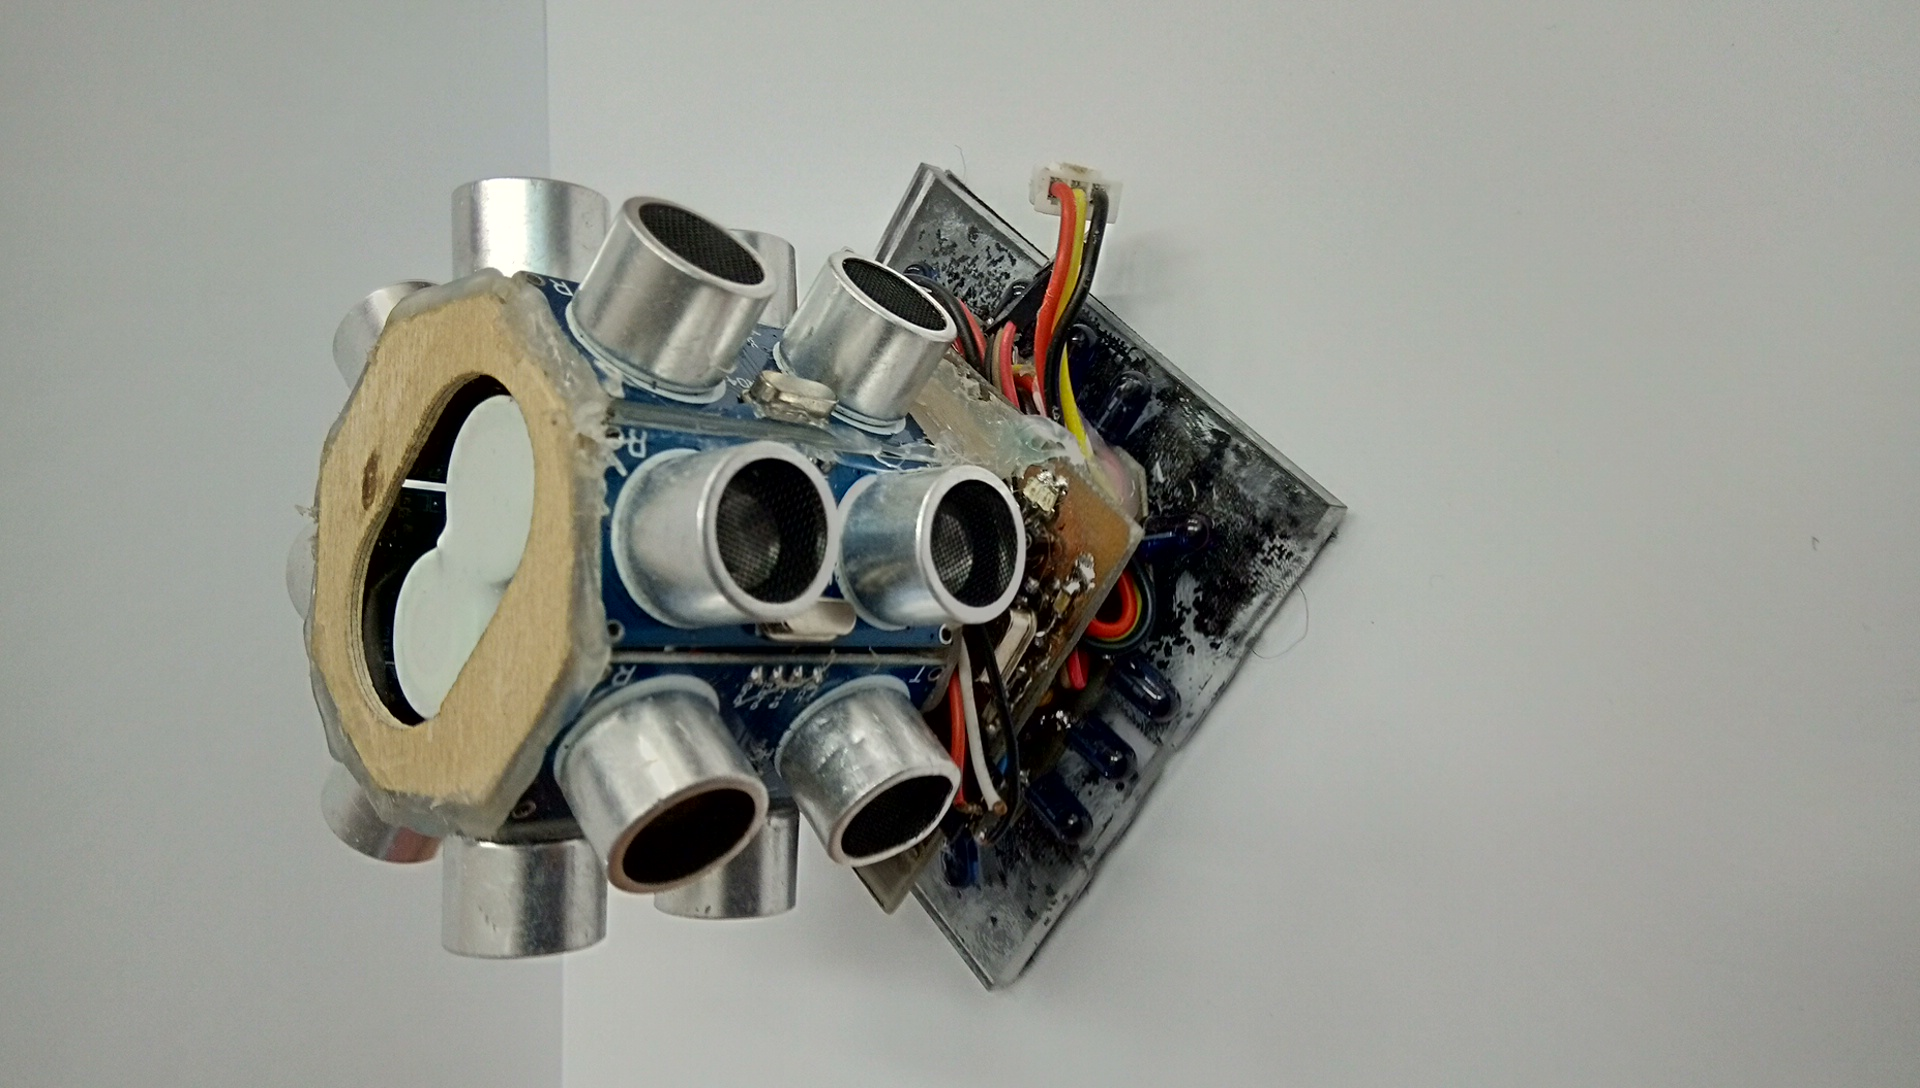
\includegraphics[width=250px, angle = 0, scale = 0.7]{img/Vysilac2.jpg}
        \end{center}
        \caption{Vysílač}
        \label{fig: Ultrasonic}
    \end{small}
\end{figure}


\subsubsection{Přijímač}
Přijímač sestává ze singleplayerové verze, kruhu osmi IR přijímačů TSOP4840 a řídící jednotky.
Všechny HC-SR04 mají znefunkčněný vysílač.
Když procesor přijme z~IR přijímačů signál, započne měřit čas a odešle vysílací puls do HC-SR04, poté již jen čeká než se změní hodnota některého z~Echo pinů na HC-SR04.
V~okamžiku, kdy se tak stane, procesor ukončí měření času a zaznamená si, ze kterého HC-SR04 změna přišla.
Díky tomu je schopen senzor zjistit nejen vzdálenost od vysílače, ale i přibližný směr k~němu.
Cokoliv, co přijde po první změně nás nezajímá, protože se jedná o~náhodný odraz od objektů v~prostředí.

\section{Sběrač ultrazvukových senzorů}\label{Sberac}
Tento senzor používá řídící elektroniku singleplayerového řešení všesměrového senzoru.
Hlavní rozdíl oproti němu je možnost libovolného umístění senzorů HC-SR04 na robota.
Důvodem tvorby tohoto senzoru je časová náročnost měření jednotlivých senzorů, která může razantně ovlivnit reakční dobu robota.
Senzor je navíc oproti singlplayerovému řešení schopen po softwarovém zapnutí této funkce odesílat interupt signál při překročení nastavené meze přiblížení pro některý z~HC-SR04.
	
	%%% Závěr
	\newpage
\chapter*{Závěr}
\addcontentsline{toc}{chapter}{Závěr}

Ke dni odevzdání textové části práce je funční Omni-ultra, všesměrový ultrazvukový senzor a~Janus protocol jako takový.
Ve vývoji se nachází knihovna pro práci s~jednotlivími senzory.
Začátečníkům z~robotických kroužků na SPŠ Sokolské Brno \cite{sokolska} a pobočce DDM Helceletova Brno -- Robotárně \cite{robotarna} se tak do rukou dostává fungující systém se zatím omezeným množstvím senzorů, se kterými mohou experimentovat.
Pokročilejší uživatelé pak mají možnost požít ekosystém pro vytvoření vlastních senzorů a modulů.
Všechny mnou vytvořené součásti ekosystému jsou volně dostupné jako Open Source, na Githubu \cite{protocol}.

%I~přesto asi nejdůležitější výsledek, který si z~práce odnáším já osobně, jsou zkušenosti s~většími komplexními projekty, v~porovnání s~mými dosavadními získané hlavně prací na samostatných malých projektech.

Janus protocol a hlavně jednotky, které na něm operují, se mají stále kam rozvíjet a to jak kvalitativně, tak i kvantitativně.

Do budoucna mám v~plánu dodělat kompletní a jednoduše srozumitelnou dokumentaci jak pro celý protokol, tak pro jednotlivé senzory.
Především kvůli tomu, aby si již zkušenější uživatelé mohli přidávat sami další senzory do ekosystému a poskytovali tím méně zkušeným uživatelům dostupnou sadu senzorů pro vlastní experimentování.
Pro pohodlnost práce plánuji přidat modul pro Sigrok (program pro analýzu dat z~logického analyzéru), určený k~rychlé kontrole dat na sběrnici.

	
	\newpage
	\printbibliography[title=Literatura]
	\addcontentsline{toc}{chapter}{Literatura}
	
	\listoffigures
	\addcontentsline{toc}{chapter}{Seznam obrázků}
	
	\listoftables
	\addcontentsline{toc}{chapter}{Seznam tabulek}
	
	\listoflistedequation
	\addcontentsline{toc}{chapter}{Seznam rovnic}
	
\end{document}
